\begin{figure}[tbh]
		\centering
		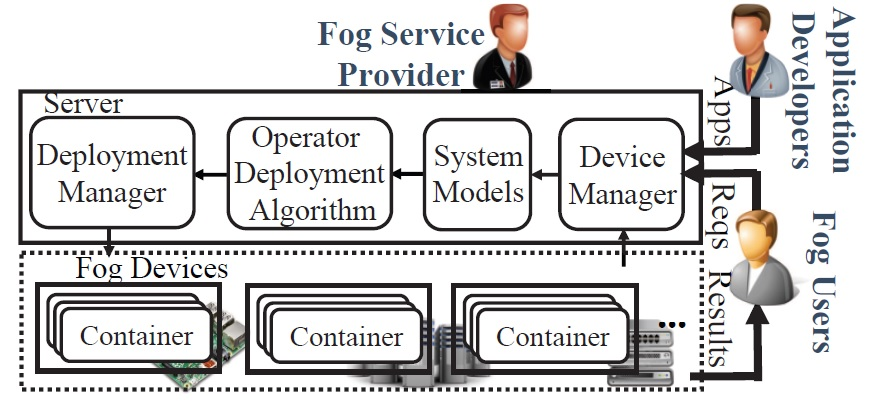
\includegraphics[width=0.40\textwidth]{fig/architecture.eps}
		\caption{High-level system architecture with a network of MANEs.}
\vspace{-0.1cm}
		\label{architecture} 
\end{figure}

\section{System Architecture} \label{sec:architecture}

%The considered system is composed of an ONOS controller, a video server, multiple video clients, and several MANEs as shown in Fig.~\ref{architecture}. The ONOS controller forms a control plane disassociated from data plane among P4 switches. Using the knowledge on the network topology and available resources, the ONOS controller determines the best routes from servers through MANEs to clients. Once the streaming starts, each MANE drops the scalable video packets when necessary.
%
%The life cycle of the video streaming sessions is as follows. First, the receiver sends a request to the server, and the server sends the encoded video streams through the MANEs. During transmissions, the ONOS controller communicates with all MANEs to set up the outgoing port for packets. When the network topology changes, the ONOS controller informs every MANE for the alternative paths immediately. The ONOS controller may also fine-tune the video quality levels of different users for optimal overall quality.
